\documentclass[a4paper,12pt]{article}

\usepackage[utf8]{inputenc}
\usepackage[T1]{fontenc}
\usepackage[english]{babel}

\usepackage{listings}
\usepackage{xcolor}
\usepackage{courier}

\usepackage{graphicx}
\usepackage{tikz}
\usetikzlibrary{arrows.meta, positioning, shapes.geometric}

\lstset{
    basicstyle=\ttfamily\small,
    keywordstyle=\color{blue},
    commentstyle=\color{gray},
    stringstyle=\color{red},
    numbers=left,
    numberstyle=\tiny,
    stepnumber=1,
    frame=single,
    breaklines=true,
    tabsize=4,
    showstringspaces=false,
    captionpos=b
}

\title{\textbf{MPI File Transfer Program Report}}
\author{Hoang Minh Quan\\ID 23BI14371}
\date{\today}

\begin{document}

\maketitle
\tableofcontents
\newpage

\section{Introduction}

This report presents an MPI-based file transfer program implemented in C++.  
The goal of the program is to allow one MPI process (the \texttt{ROOT} process) to read a file and distribute its contents to all other MPI processes using the \texttt{MPI\_Bcast} communication primitive.

Each non-root process receives the file and writes it to a new local file named according to its MPI rank.

\section{Program Objectives}

The application fulfills the following objectives:

\begin{itemize}
    \item The ROOT process reads the name and contents of a file.
    \item The file name and its length are broadcast to all MPI processes.
    \item The file data buffer is broadcast to all MPI processes.
    \item Each receiver process writes the received data into a new file named:
    \[
        \texttt{received\_rankX\_filename}
    \]
\end{itemize}

The program requires at least 2 MPI processes: 
\begin{itemize}
    \item One sender (rank 0)
    \item One or more receivers (ranks 1, 2, \dots)
\end{itemize}

\section{System Illustration}

Figure~\ref{fig:system} shows a high-level view of the MPI file transfer system.  
Rank 0 acts as the sender: it reads the input file and broadcasts its contents to all other ranks, which act as receivers.

\begin{figure}[h!]
    \centering
    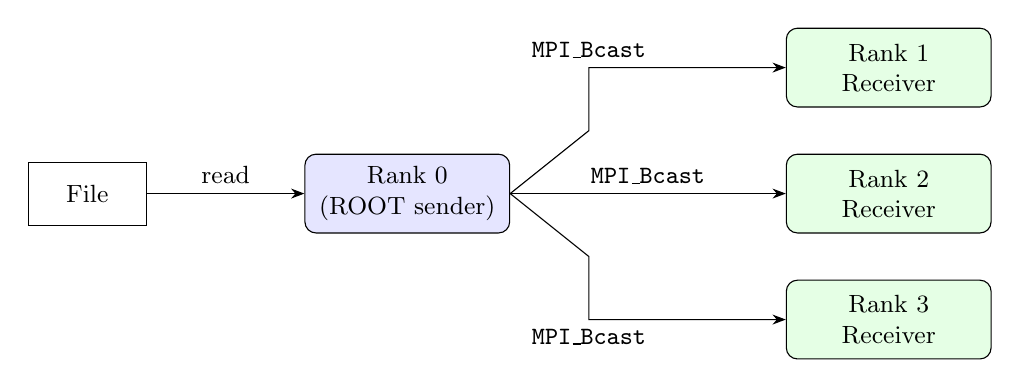
\begin{tikzpicture}[
        node distance=1.8cm and 1.8cm,
        every node/.style={font=\small},
        proc/.style={rectangle, rounded corners, draw, minimum width=2.6cm, minimum height=1cm, align=center},
        >=Stealth
    ]
        \node[proc, fill=blue!10] (root) {Rank 0 \\ (ROOT sender)};
        \node[proc, fill=green!10, right=3.5cm of root, yshift=1.6cm] (r1) {Rank 1 \\ Receiver};
        \node[proc, fill=green!10, right=3.5cm of root] (r2) {Rank 2 \\ Receiver};
        \node[proc, fill=green!10, right=3.5cm of root, yshift=-1.6cm] (r3) {Rank 3 \\ Receiver};

        \node[rectangle, draw, minimum width=1.5cm, minimum height=0.8cm, left=2cm of root] (file) {File};

        \draw[->] (file) -- node[above]{read} (root);

        \draw[->] (root.east) -- ++(1,0.8) |- node[above]{\texttt{MPI\_Bcast}} (r1.west);
        \draw[->] (root.east) -- node[above]{\texttt{MPI\_Bcast}} (r2.west);
        \draw[->] (root.east) -- ++(1,-0.8) |- node[below]{\texttt{MPI\_Bcast}} (r3.west);

    \end{tikzpicture}
    \caption{High-level illustration of the MPI file transfer system.}
    \label{fig:system}
\end{figure}


\section{Source Code}

The full source code of the MPI program is shown below.

\begin{lstlisting}[language=C++, caption={MPI File Transfer Source Code}]
#include <mpi.h>
#include <iostream>
#include <fstream>
#include <vector>
#include <string>

int main(int argc, char** argv) {
    MPI_Init(&argc, &argv);

    int rank, size;
    MPI_Comm_rank(MPI_COMM_WORLD, &rank);
    MPI_Comm_size(MPI_COMM_WORLD, &size);

    const int ROOT = 0;

    if (size < 2) {
        if (rank == ROOT) {
            std::cerr << "Need at least 2 MPI processes (1 sender + 1 receiver)." << std::endl;
        }
        MPI_Finalize();
        return 1;
    }

    std::string filename;
    std::vector<char> nameBuf;
    int nameLen = 0;

    if (rank == ROOT) {
        if (argc < 2) {
            std::cerr << "Usage: mpirun -np <n> ./mpi_file_transfer <file_to_send>\n";
            MPI_Abort(MPI_COMM_WORLD, 1);
        }
        filename = argv[1];

        nameBuf.assign(filename.begin(), filename.end());
        nameBuf.push_back('\0');
        nameLen = static_cast<int>(nameBuf.size());
    }

    MPI_Bcast(&nameLen, 1, MPI_INT, ROOT, MPI_COMM_WORLD);

    if (rank != ROOT) {
        nameBuf.resize(nameLen);
    }

    MPI_Bcast(nameBuf.data(), nameLen, MPI_CHAR, ROOT, MPI_COMM_WORLD);

    if (rank != ROOT) {
        filename = std::string(nameBuf.data());
    }

    int fileSize = 0;
    std::vector<char> buffer;

    if (rank == ROOT) {
        std::ifstream in(filename, std::ios::binary);
        if (!in.is_open()) {
            std::cerr << "Rank " << rank << ": cannot open file '" << filename << "' for reading.\n";
            MPI_Abort(MPI_COMM_WORLD, 1);
        }

        in.seekg(0, std::ios::end);
        fileSize = static_cast<int>(in.tellg());
        in.seekg(0, std::ios::beg);

        buffer.resize(fileSize);
        if (fileSize > 0) {
            in.read(buffer.data(), fileSize);
        }
        in.close();

        std::cout << "Rank " << rank << ": read " << fileSize
                  << " bytes from '" << filename << "'.\n";
    }

    MPI_Bcast(&fileSize, 1, MPI_INT, ROOT, MPI_COMM_WORLD);

    if (fileSize == 0) {
        if (rank != ROOT) {
            std::cerr << "Rank " << rank
                      << ": received file size 0, nothing to write.\n";
        }
        MPI_Finalize();
        return 0;
    }

    if (rank != ROOT) {
        buffer.resize(fileSize);
    }

    MPI_Bcast(buffer.data(), fileSize, MPI_CHAR, ROOT, MPI_COMM_WORLD);

    if (rank != ROOT) {
        std::string outName = "received_rank"
                              + std::to_string(rank)
                              + "_" + filename;

        std::ofstream out(outName, std::ios::binary);
        if (!out.is_open()) {
            std::cerr << "Rank " << rank
                      << ": cannot open '" << outName << "' for writing.\n";
            MPI_Abort(MPI_COMM_WORLD, 1);
        }

        out.write(buffer.data(), fileSize);
        out.close();

        std::cout << "Rank " << rank << ": wrote " << fileSize
                  << " bytes to '" << outName << "'.\n";
    }

    MPI_Finalize();
    return 0;
}
\end{lstlisting}

\section{How to Compile}

To compile the program on a system with MPI installed:

\begin{verbatim}
mpic++ mpi_file_transfer.cpp -o mpi_file_transfer
\end{verbatim}

\section{How to Run the Program}

Run the program with at least 2 processes:

\begin{verbatim}
mpirun -np 4 ./mpi_file_transfer example.bin
\end{verbatim}

Expected behavior:

\begin{itemize}
    \item Rank 0 reads \texttt{example.bin}.
    \item All ranks receive the file through MPI broadcast.
    \item Ranks 1, 2, 3 write:
    \begin{verbatim}
    received_rank1_example.bin
    received_rank2_example.bin
    received_rank3_example.bin
    \end{verbatim}
\end{itemize}

\section{Conclusion}

This MPI application demonstrates how to efficiently distribute file data from one process to all others using collective communication.

The program:
\begin{itemize}
    \item Uses \texttt{MPI\_Bcast} for distributing metadata and file contents.
    \item Avoids sending the file multiple times by using a single collective operation.
    \item Ensures each process receives an identical copy of the input file.
\end{itemize}

This approach is well-suited for small to medium file sizes and showcases a clean example of using MPI for data distribution.

\end{document}
